\clearpage
\appendix
\setcounter{figure}{0}
\setcounter{table}{0}
\renewcommand{\thefigure}{S\arabic{figure}}
\renewcommand{\thetable}{S\arabic{table}}

\section*{Supplementary material}

This appendix carries the implementation detail removed from the main paper. It adds no result and
changes no claim; every number below is a property of an asset or an operator, not of a trained
model.

\section{The CSC operator}
\label{sup:csc}

\paragraph{Baking $T_i$.}
For each part $i$ and each texel centre $q=((a{+}\tfrac12)/K,(b{+}\tfrac12)/K)$ we find the first
chart triangle containing $q$ among the $32$ nearest chart-triangle centroids (KD-tree), take its
2D barycentrics $\beta$, and set $T_i[b,a]=\sum_k\beta_kX_k$ over the face's three template
vertices. Texels covered by no triangle are filled by clipped-barycentric projection onto the
nearest candidate, so the texture is finite and smooth everywhere and never reads garbage. Texels
claimed by more than one triangle, or by none, are flagged ambiguous and the flag is dilated by one
texel because the bilinear stencil is $2{\times}2$.

\paragraph{The read.}
$\Phi(i,u,v)$ is one 3D \texttt{grid\_sample} into a $(1,3,24,K,K)$ volume at
$\xi=2u-1$, $\eta=2v-1$, $\zeta=(2i-1)/24-1$ with \texttt{align\_corners=False}; $\zeta$ lands
exactly on the centre of slice $i{-}1$, so interpolation along the part axis is a no-op and part
selection is exact. $\Phi$ must run in \texttt{fp32}: under \texttt{bf16} autocast a $u\in[0,1]$
resolves to about one texel and the gradient signal is destroyed, so the operator disables autocast
for itself.

\paragraph{Validation gates ($K{=}512$, \textsc{v2} charts).}
(G1) Round-trip against exact barycentric XYZ on $200$k random surface points: on the $74.5\%$ of
samples the ambiguity mask admits, median $<0.001$\,mm, p99 $0.335$\,mm, \emph{max} $63.35$\,mm ---
our own pass criterion is $\max<1$\,mm, so this gate fails on its own terms and we report it as a
thin tail on sliver triangles and texel boundaries rather than as a pass. Per region, hands are
$84.5\%$ usable, feet $88.1\%$, head only $52.3\%$ --- the last is the hidden-geometry mask of
\cref{sec:data} doing its job. (G2) Autograd $\partial\Phi/\partial(u,v)$ against float64 central
differences ($h{=}10^{-7}$): median relative error $5.21\times10^{-10}$. (G3) Ground-truth $uv$
pushed through the losses: $\mathcal{L}_{\mathrm{xyz}}=0.0135$\,mm,
$\mathcal{L}_{\mathrm{grad}}=0.0056$\,mm.

\section{Orientation recipe ladder}
\label{sup:ladder}

\begin{table}[h]
\setlength{\tabcolsep}{4pt}
\centering\footnotesize
\begin{tabular}{@{}lcccc@{}}
\toprule
Configuration & geo$^\circ$ & $\Delta$ & part acc & uv $L_1$ \\
\midrule
single $6$D head, flat LR      & 9.01 & --- & 0.9621 & 0.0263 \\
$+$ per-part rotation head     & 8.48 & $-0.53$ & 0.9611 & 0.0266 \\
\quad alt.\ $+$ LLRD, $3\mathrm{e}{-}4$ \emph{(shipped)} & 8.05 & $-0.43$ & 0.9619 & 0.0259 \\
\quad alt.\ $+$ LLRD, $1\mathrm{e}{-}3$ & 7.86 & $-0.62$ & 0.9659 & 0.0251 \\
$+$ 58k$\rightarrow$120k \emph{($1\mathrm{e}{-}3$ branch)} & 7.30 & $-0.56$ & 0.9692 & 0.0228 \\
\bottomrule
\end{tabular}
\caption{Matched step 58k, \textbf{oracle} gather: the rotation channel is taken at the
ground-truth part, which measures the head in isolation and is optimistic --- on the one lineage
where we measured both, by $0.65^\circ$ ($7.30^\circ$ oracle against $7.95^\circ$ end-to-end). It
is therefore \emph{not} comparable with the deployment numbers in the main paper, a different
readout of a different lineage. ``part acc'' is $24$-way part accuracy, ``uv $L_1$'' mean
chart-unit error, both on foreground. The two LLRD rows are \emph{alternatives}, each measured
against the row above, so $\Delta$ does not telescope, and the last rung continues the branch we do
\emph{not} ship. No external baseline; single run per row.}
\label{tab:orient}
\end{table}

\begin{figure}[h]
\centering
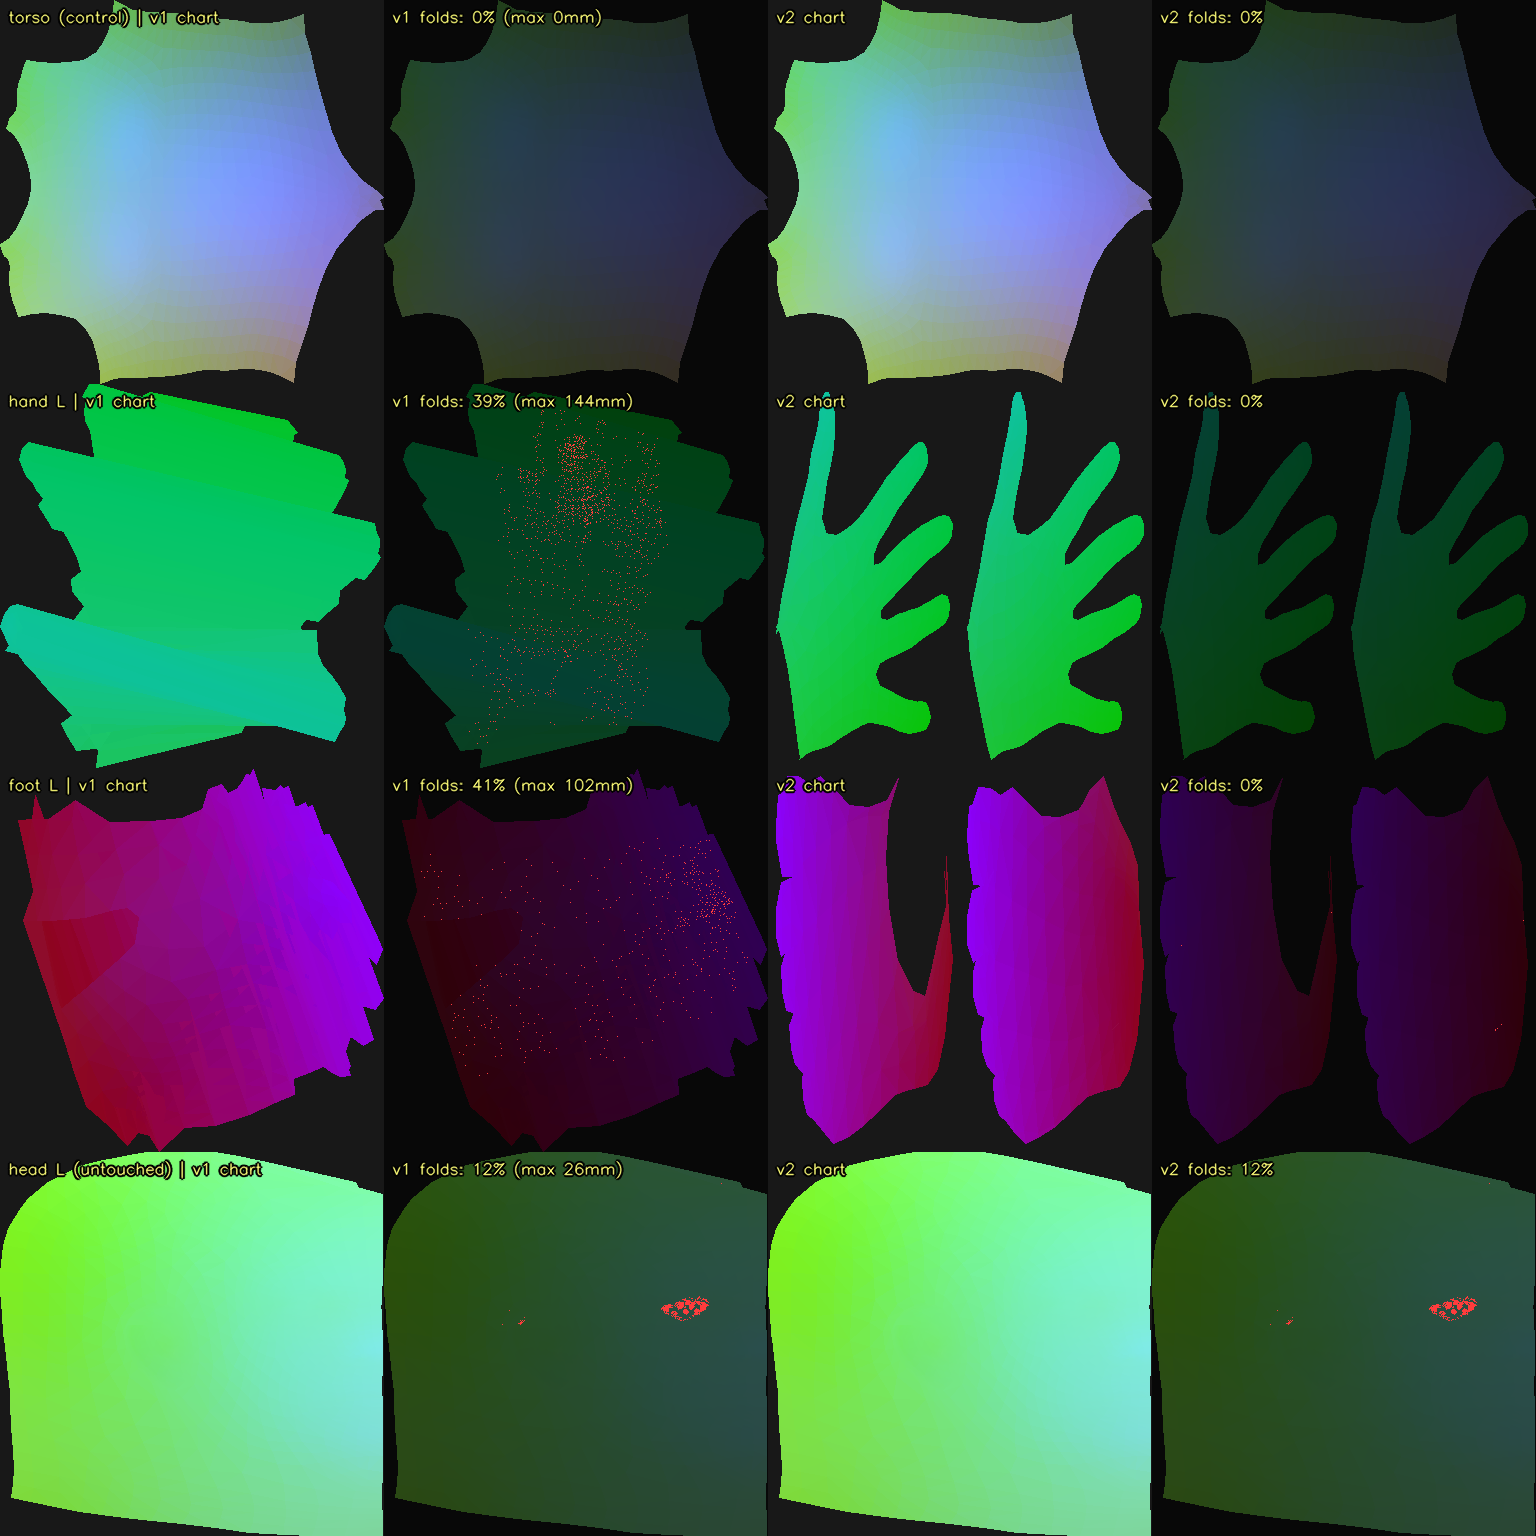
\includegraphics[width=\linewidth]{figs/fig_charts.png}
\caption{\textbf{The official DP24 atlas is non-injective on hands and feet.} Rows: torso
(control), hand, foot, head half (unchanged). Columns: the \textsc{v1} chart shaded by template
position; surface samples claimed by more than one triangle, in red; the \textsc{v2} chart; its
overlay. Annotations are chart-area weighted and quote the \emph{worst} collision; the text quotes
surface-sample fractions and the median.}
\label{fig:charts}
\end{figure}

\section{Chart re-flattening: rejected alternatives}
\label{sup:charts}

Tutte/Floater mean-value embedding gives a \emph{guaranteed} fold-free chart (exactly $0\%$ on
feet) but crushes the extremities: $409$ of $1538$ hand triangles collapse below $10^{-9}$ chart
area --- injective in exact arithmetic, degenerate in float64 --- and the texture round-trip
degrades to a median of $0.203$\,mm against $0.010$\,mm for the sheet split, i.e.\ the chart loses
resolution exactly where the artifacts were. LSCM folds outright ($122$ flipped triangles). On the
head, a spherical parameterisation is worse than the original ($69\%$ overlap) and the sheet split
reaches $32\%$; the residual there is dominated by geometry hidden \emph{inside} the part rather
than by the flattening, which is why the head is masked rather than re-cut.

\section{The fixed ground-truth canvas}
\label{sup:canvas}

Both the ground-truth canvas and the model input are axis-aligned squares in source-frame pixels,
so the map from the network's output frame into the canvas is a pure scale-and-translate affine
available in closed form. With $g_{\mathrm{side}},g_{x_0},g_{y_0}$ the canvas window and
$i_{\mathrm{size}},i_{x_0},i_{y_0}$ the input window,
\begin{equation*}
  s=\frac{g_{\mathrm{side}}}{i_{\mathrm{size}}},\qquad
  t_d=\frac{2(g_{d_0}-i_{d_0})}{i_{\mathrm{size}}}+s-1 \;\; (d\in\{x,y\}),
\end{equation*}
and $\theta_{\mathrm{warp}}=[\,[s,0,t_x],[0,s,t_y]\,]$ is fed to one \texttt{affine\_grid} /
\texttt{grid\_sample} pair per head with \texttt{align\_corners=False}; the expression is
independent of the two raster resolutions. The $144$-channel rotation field is warped in
\texttt{bf16} (fp32 activations would be $4.8$\,GB at batch $32$) and upcast only after the
six-channel gather; UV is warped in \texttt{fp32} for the reason in \cref{sup:csc}. The $4\%$ margin
between the crop's $1.25\times$ lower bound and the canvas's $1.2\times$ matters: without it,
integer rounding of the crop window left a ring of ground-truth pixels with no image support in
$2$ of $300$ sampled instances.

\section{Hidden geometry}
\label{sup:hidden}

The hidden-face set is $2176$ eyeball faces (two closed components, exactly $1088$ per eye) plus
$1694$ interior head faces ($847$ per half), the latter found with M\"oller--Trumbore: an outward
ray from the face centroid must re-hit \emph{head} geometry within $10$\,cm. Requiring the hit to be
head geometry is what removes the under-chin-to-chest false positives. Together they are $1.01\%$ of
head pixels and $0.106\%$ of foreground.

\section{Occlusion holdout}
\label{sup:holdout}

$\mathrm{md5}(\text{seq})\bmod 50=0$ selects $29$ of $2211$ sequences and $59$ of $5417$ shards
($1.1\%$), spanning all four MAMMA sub-datasets (harmony4d $3$, inter-x $20$, interactions $5$,
latindance10 $1$). Shard names embed sequence ids, so the exclusion is exact and there is no
temporal leakage between train and probe.

\section{Leffa cross-evaluation}
\label{sup:leffa}

Leffa's published numbers come from VtonEval, whose LPIPS is torchmetrics/SqueezeNet after a
1024-px resize, whereas MCLD's \texttt{evaluate.py} (and \cref{tab:mcld}) use the \texttt{lpips}
package's AlexNet LPIPS at the stated resolution; the agreement of shared baseline rows across the
two papers proves only that both copied those rows from their sources. Re-scoring our own outputs
under VtonEval's definitions gives arm~B $0.0891$/$0.1077$ LPIPS at $256$/$512$ and arm~A
$0.0961$/$0.1149$. To remove any dependence on published numbers we then ran Leffa's released
\texttt{pose\_transfer.pth} ourselves (SDXL-inpainting base, their DensePose R-50, $50$ steps,
guidance $2.5$, seed $42$) and scored Leffa and both arms on the same $1499$ pairs under both
harnesses:

\begin{figure}[h]\centering
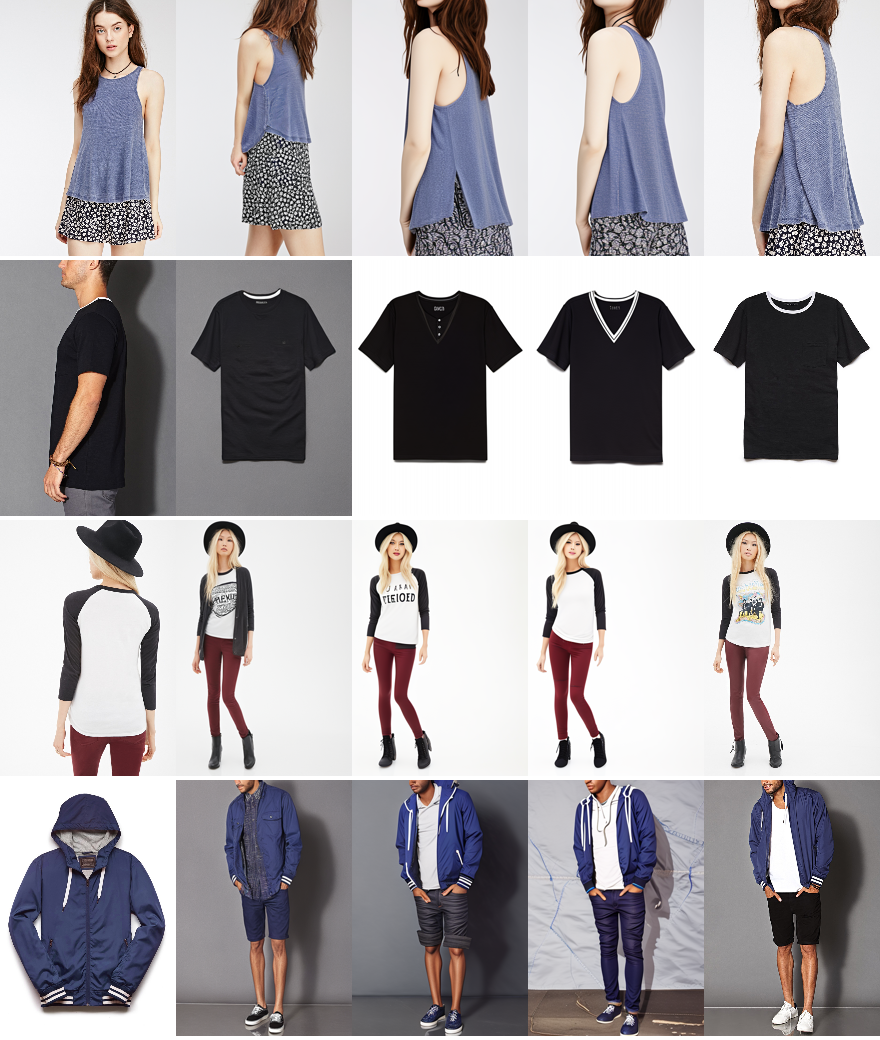
\includegraphics[width=\linewidth]{figs/fig_leffa.png}
\caption{Source, Leffa, arm~A, arm~B, ground truth. Rows are selected \emph{by} per-image LPIPS,
not curated: the two largest margins over Leffa, the median case, and the case where Leffa wins
most --- there arm~B emits a background artifact, and we include it for that reason.}
\label{fig:leffa}
\end{figure}

